\documentclass[10pt]{extarticle}

\usepackage[utf8]{inputenc}
\usepackage[T1]{fontenc}
\usepackage{textcomp}

\usepackage{url}

% \usepackage{hyperref}
% \hypersetup{
%     colorlinks,
%     linkcolor={black},
%     citecolor={black},
%     urlcolor={blue!80!black}
% }

\usepackage{graphicx}
\usepackage{float}
\usepackage[usenames,dvipsnames]{xcolor}

% \usepackage{cmbright}

\usepackage{amsmath, amsfonts, mathtools, amsthm, amssymb}
\usepackage{mathrsfs}
\usepackage{cancel}

% horizontal rule
\newcommand\hr{
    \noindent\rule[0.5ex]{\linewidth}{0.5pt}
}

\usepackage{tikz}
\usepackage{tikz-cd}

% theorems
\usepackage{thmtools}
\usepackage[framemethod=TikZ]{mdframed}
\mdfsetup{skipabove=1em,skipbelow=0em, innertopmargin=5pt, innerbottommargin=6pt}

\theoremstyle{definition}

\makeatletter

\declaretheoremstyle[headfont=\bfseries\sffamily, bodyfont=\normalfont, mdframed={ nobreak } ]{thmgreenbox}
\declaretheoremstyle[headfont=\bfseries\sffamily, bodyfont=\normalfont, mdframed={ nobreak } ]{thmredbox}
\declaretheoremstyle[headfont=\bfseries\sffamily, bodyfont=\normalfont]{thmbluebox}
\declaretheoremstyle[headfont=\bfseries\sffamily, bodyfont=\normalfont]{thmblueline}
\declaretheoremstyle[headfont=\bfseries\sffamily, bodyfont=\normalfont, numbered=no, mdframed={ rightline=false, topline=false, bottomline=false, }, qed=\qedsymbol ]{thmproofbox}
\declaretheoremstyle[headfont=\bfseries\sffamily, bodyfont=\normalfont, numbered=no, mdframed={ nobreak, rightline=false, topline=false, bottomline=false } ]{thmexplanationbox}


\declaretheorem[numberwithin=chapter, style=thmgreenbox, name=Definition]{definition}
\declaretheorem[sibling=definition, style=thmredbox, name=Corollary]{corollary}
\declaretheorem[sibling=definition, style=thmredbox, name=Proposition]{prop}
\declaretheorem[sibling=definition, style=thmredbox, name=Theorem]{theorem}
\declaretheorem[sibling=definition, style=thmredbox, name=Lemma]{lemma}



\declaretheorem[numbered=no, style=thmexplanationbox, name=Proof]{explanation}
\declaretheorem[numbered=no, style=thmproofbox, name=Proof]{replacementproof}
\declaretheorem[style=thmbluebox,  numbered=no, name=Exercise]{ex}
\declaretheorem[style=thmbluebox,  numbered=no, name=Example]{eg}
\declaretheorem[style=thmblueline, numbered=no, name=Remark]{remark}
\declaretheorem[style=thmblueline, numbered=no, name=Note]{note}

\renewenvironment{proof}[1][\proofname]{\begin{replacementproof}}{\end{replacementproof}}

\AtEndEnvironment{eg}{\null\hfill$\diamond$}%

\newtheorem*{uovt}{UOVT}
\newtheorem*{notation}{Notation}
\newtheorem*{previouslyseen}{As previously seen}
\newtheorem*{problem}{Problem}
\newtheorem*{observe}{Observe}
\newtheorem*{property}{Property}
\newtheorem*{intuition}{Intuition}


\usepackage{etoolbox}
\AtEndEnvironment{vb}{\null\hfill$\diamond$}%
\AtEndEnvironment{intermezzo}{\null\hfill$\diamond$}%




% http://tex.stackexchange.com/questions/22119/how-can-i-change-the-spacing-before-theorems-with-amsthm
% \def\thm@space@setup{%
%   \thm@preskip=\parskip \thm@postskip=0pt
% }

\usepackage{xifthen}

\def\testdateparts#1{\dateparts#1\relax}
\def\dateparts#1 #2 #3 #4 #5\relax{
    \marginpar{\small\textsf{\mbox{#1 #2 #3 #5}}}
}

\def\@lesson{}%
\newcommand{\lesson}[3]{
    \ifthenelse{\isempty{#3}}{%
        \def\@lesson{Lecture #1}%
    }{%
        \def\@lesson{Lecture #1: #3}%
    }%
    \subsection*{\@lesson}
    \testdateparts{#2}
}

% fancy headers
\usepackage{fancyhdr}
\pagestyle{fancy}

% \fancyhead[LE,RO]{Gilles Castel}
\fancyhead[RO,LE]{\@lesson}
\fancyhead[RE,LO]{}
\fancyfoot[LE,RO]{\thepage}
\fancyfoot[C]{\leftmark}
\renewcommand{\headrulewidth}{0pt}

\makeatother

% figure support (https://castel.dev/post/lecture-notes-2)
\usepackage{import}
\usepackage{xifthen}
\pdfminorversion=7
\usepackage{pdfpages}
\usepackage{transparent}
\newcommand{\incfig}[1]{%
    \def\svgwidth{\columnwidth}
    \import{./figures/}{#1.pdf_tex}
}

% %http://tex.stackexchange.com/questions/76273/multiple-pdfs-with-page-group-included-in-a-single-page-warning
\pdfsuppresswarningpagegroup=1

\author{Gilles Castel}

\makeindex

\title{Tutorium MfP4 - SoSe 25}
\author{zur Vorlesung von PD Dr. Holtkamp}
\date{\today} % Replace with \today to show the current date

\begin{document}
\let\temp\phi
\let\phi\varphi
\let\varphi\temp
\maketitle

\definecolor{tcol_CNT1}{HTML}{72E094} % First color for Contents
\definecolor{tcol_CNT2}{HTML}{24E2D6} % Second color for Contents
\definecolor{tcol_CNV1}{HTML}{8E44AD} % First color for Conventions
\definecolor{tcol_CNV2}{HTML}{A10B49} % First color for Conventions

\begin{tcolorbox}[enhanced,
    title=Inhaltsverzeichnis,
    fonttitle=\fontsize{20}{24}\sffamily\bfseries\selectfont,
    coltitle=black,
    fontupper=\sffamily,
    attach boxed title to top center={yshift=10pt},
    boxed title style={frame hidden,
        interior style={left color=tcol_CNT1!0,right color=tcol_CNT2!0},
        frame style={left color=tcol_CNT1!0!black,right color=tcol_CNT2!0!black},
        height=24pt,bean arc,drop fuzzy shadow
    },
    top=2mm,bottom=2mm,left=2mm,right=2mm,
    before skip=20mm,after skip=20mm,
    drop fuzzy shadow,breakable]
%
\makeatletter
\@starttoc{toc}
\makeatother
\end{tcolorbox}

\begin{tcolorbox}[enhanced,
    title=Konventionen,
    fonttitle=\large\sffamily\bfseries\selectfont,
    boxrule=2pt,left=2pt,right=2pt,
    attach boxed title to top left,
    top=2mm,bottom=2mm,left=2mm,right=2mm,
    before skip=10mm,after skip=10mm]
%
\begin{itemize}
\item Wir schreiben für einen Körper $\K$ kurz $\K^\ast := \K \exc \{0\}$.
\item Real- und Imaginärteil werden mit $\Re(\cdot)$ respektive $\Im(\cdot)$ bezeichnet, das Bild einer Abbildung $f$ hingegen mit $\im (f)$.
\item Echte Teilmengen tragen das Symbol $\subset$, allgemeine Teilmengen das Symbol $\sub$.
\end{itemize}
\end{tcolorbox}
Dies sind meine Tutoriumsnotizen für Mathe für Physiker 4. Falls Ihr Fehler findet, sagt immer gerne Bescheid. Allgemein sind die Notizen oft schnell von mir für meine eigene Tutoriumsvorbereitung getippt, erwartet also bitte kein voll ausgearbeitetes \LaTeX-Skript.
\newpage 
\sloppy
\section{Tutorium 10.04.25}
\label{sec:10_04_25}

\subsection{Organisatorisches}
\begin{itemize}
\item Festlegung des allgemeinen Tutoriumtermins. Ort: Voraussichtlich wieder Geomatikum, wenn Raum verfügbar.
\item Fahrplan MfP4: Differentialgeometrie, Funktionentheorie, Funktionalanalysis
\item Wünsche für das Tutorium? Vergleich letzte Semester, konkrete Vorstellungen, etc.
\item MathNet-Wolke, Moodle, Homepage, Telegram-Gruppe
\end{itemize}

\subsection{Literaturempfehlungen}
Zur Differentialgeometrie kennt ihr bereits meine Empfehlungen von letztem Semester.
Zur Funktionentheorie:
\begin{itemize}
\item Jänich, \href{https://link.springer.com/book/10.1007/3-540-35015-2}{Funktionentheorie}: Sehr angenehm zu lesendes Buch, vor allem, wenn man vielleicht auch an gut geschriebenen Büchern und Anekdoten Spaß hat. 
\item Salamon, \href{https://link.springer.com/book/10.1007/978-3-0348-0169-0}{Funktionentheorie}: Das Buch basiert auf Ahlfors, Complex Analysis, einem beachtlich guten Standardwerk im englischen Raum. Etwas trockener als Jänich, eher im typischen Mathe-Stil.
\item Needham, \href{https://umv.science.upjs.sk/hutnik/NeedhamVCA.pdf}{Visual Complex Analysis}: Das (englischsprachige) Buch kann man am besten nebenher lesen, wenn man sich für die geometrische Intuition hinter der Funktionentheorie interessiert.
\end{itemize}
Zur Funktionalanalysis:
Hier ist das Skript kaum zu schlagen, da die Themenwahl wirklich sehr speziell auf das Notwendigste für die Physik gelegt wurde. Die meisten Mathebücher würden die Konzepte aus dem zweiten Semesterteil auf zwei ganze Semester aufteilen. Und dazu kommt noch mehr Maßtheorie\dots. Nichtsdestotrotz, ein bisschen was fällt mir ein:
\begin{itemize}
\item Kaballo, \href{https://link.springer.com/book/10.1007/978-3-662-54748-9}{Grundkurs Funktionalanalysis}: Das Buch ist aus einem MfP-ähnlichen Modul entstanden und daher einigermaßen geeignet. Allgemein ist das Buch relativ nett geschrieben.
\item Hall, \href{https://link.springer.com/book/10.1007/978-1-4614-7116-5}{Quantum Theory for Mathematicians}: Hier wird die Funktionalanalysis aus Sicht der Physik mit mittelmäßigem mathematischen Anspruch betrachtet. Mathematisch streng veranlagte Leute können mit dem Buch oft nicht so viel anfangen, manchen gereicht es aber auch zur Rettung. Einfach mal reinlesen :)
\end{itemize}
Im Allgemeinen ist MfP4 meiner Erfahrung nach, vor allem wenn noch Differentialgeometrie abgefragt wird, sehr gut machbar, vor allem im Vergleich zu den sehr dichten MfP2- und MfP3-Modulen. Erfahrungsgemäß mögen viele die Funktionentheorie sehr und können damit gut umgehen. Funktionalanalysis fällt hingegen meist schwer, da das Thema vielen weniger intuitiv scheint. Im besten Fall findet man aber an beidem Gefallen, im schlimmsten Fall kommt man mit DiffGeo und Funktionentheorie sicher durch die Klausur.



\section{Tutorium 17.04.25}
\label{sec:17_04_25}

\subsection{Wiederholung - Komplexe Zahlen}
Mit Sicherheit erinnert ihr euch noch gut an die komplexen Zahlen:
\begin{definition}{Komplexe Zahlen}{komplexezahlen}
Der Körper $(\C, +, \cdot)$ mit
\begin{equation}
\C := \{(a,b) \in \R \mid a,b \in \R\}
\end{equation}
und den Operationen
\begin{equation}
\begin{split}
+: \C \times \C &\to \C\\
(a,b), (c,d) &\mapsto (a,b) + (c,d) := (a+c,b+d),
\end{split}
\end{equation}
genannt Addition, und
\begin{equation}
\begin{split}
\cdot: \C \times \C &\to \C\\
(a,b),(c,d) &\mapsto (a,b) \cdot (c,d) := (ac-bd, ad+bc),
\end{split}
\end{equation}
genannt Multiplikation, nennen wir den Körper der \textbf{komplexen Zahlen}. Die Zahl $a=\Re(a,b)$ heißt \textbf{Realteil}, die Zahl $b=\Im(a,b)$ \textbf{Imaginärteil} von $z$. 
\end{definition}
Meist führt man die \textit{komplexe Einheit} $i$ ein, sodass $(a,b)=a+bi$ für $i^2:=-1$ gilt. Dies erleichtert Rechnungen, ist aber rein symbolischer Natur. Fundamental ist, dass hier ein Körper vorliegt: Sowohl $(\C, +)$ als auch $(\C^\ast, \cdot)$ sind Gruppen (das könnt ihr gerne zur Übung nachprüfen, vor allem die Inversen sollte man einmal konstruiert haben). Bereits aus MfP1 kennt ihr die \textit{komplexe Konjugation}
\begin{equation}
\begin{split}
\overline{\cdot}: \C &\to \C\\
z = a+bi &\mapsto \overline{z} := a-bi.
\end{split}
\end{equation}
Geometrisch entspricht dies einer Spiegelung an der reellen Achse. Auf $\C$ definieren wir außerdem den \textit{Absolutwert} oder \textit{Betrag} durch
\begin{equation}
\begin{split}
|\cdot |: \C &\to \C\\
z &\mapsto |z| := \sqrt{z \overline{z}} = \sqrt{\Re(z)^2+\Im(z)^2}
\end{split}
\end{equation}
mit einigen wichtigen Eigenschaften:
\begin{enumerate}[({M}1)]
\item Positivität: $|z| \geq 0$ mit $|z| = 0 \iff z=0$
\item Multiplikativität: $|z_1z_2| = |z_1||z_2|$
\item Subadditivität (Dreiecksungleichung): $|z_1+z_2| \leq |z_1| + |z_2|$.
\end{enumerate}
Sowohl die Multiplikativität als auch die Subadditivität kann man induktiv auf beliebige \red{endliche} Produkte bzw. Summen ausweiten.\\
Damit erhalten wir eine Möglichkeit, aus geometrischen Überlegungen verschiedene Formen für komplexe Zahlen herzuleiten. Ausgehend von der \textit{kartesischen Form} $z=a+bi$ definieren wir den \textbf{Radius} von $z$ als $r := |z|$. Das \textbf{(Haupt-)Argument} von $z$ ist dessen eingeschränkter Polarwinkel $\phi \in (-\pi, \pi]$, das aus trigonometrischen Überlegungen hergeleitet werden kann. Damit erhalten wir die \textit{Polarform} und mit der Eulerschen Formel auch die \textit{trigonometrische Form}:
\begin{equation}
z = r \exp(i\phi) = r(\cos \phi + i \sin \phi).
\end{equation} 
\begin{figure}[H]
\centering
\begin{tikzpicture}[scale=3]
	\draw[step=.5cm, gray, very thin, dotted] (-1.4,-1.4) grid (1.4,1.4);
	\foreach \x/\xtext in {-1, 1}
		\draw (\x,-1pt) -- (\x, 1pt) node[anchor=north] {$\xtext$};
	\foreach \y/\ytext in {-1, 1}
		\draw (-1pt, \y) -- (1pt, \y) node[anchor=east, left=2pt] {$\ytext$};
	\draw[->] (-1.5,0) -- (1.5,0);
	\draw[->] (0,-1.5) -- (0,1.5);
	\draw (0,0) circle [radius=1cm];
	\draw (.5cm,0) arc [start angle=0, end angle=40, radius=.5cm] node[right=1pt,pos=0.5] {$\phi$};
	\draw[red] (40:1cm) -- node[right=1pt, thick] {$\sin \phi = \Im(z)$} (40:1cm |- 0,0);
	\draw[blue] (0,0) -- node[below=4pt,pos=0.5, thick] {$\cos \phi = \Re(z)$} (40:1cm |- 0,0);
	\draw (0,0) -- node[above=2pt, thick] {$r$}  (40:1cm) node[black, right=1pt] {$z$};
	\filldraw[black] (40:1cm) circle [radius=0.5pt];
\end{tikzpicture}
\caption{Die Einheitskreislinie $\S^1 \hookrightarrow \C$ mit der komplexen Zahl $z=r\exp(i\phi)$.}
\end{figure}
Nicht immer ist es ganz so einfach, das Argument aus der kartesischen Form zu ermitteln. Wir illustrieren dies mal wie folgt:
\begin{figure}[H]
\centering
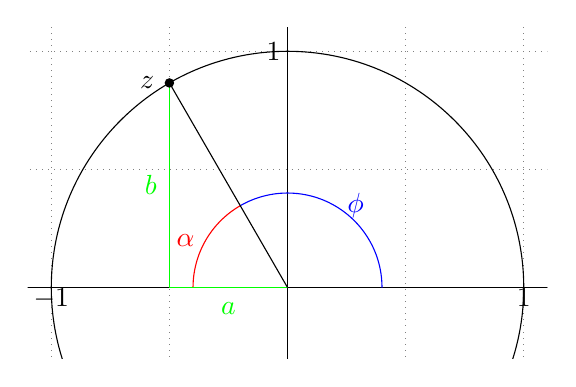
\begin{tikzpicture}[scale=3]
	\clip (-1.1, -0.3) rectangle (1.1, 1.1);
	\draw[step=.5cm, gray, very thin, dotted] (-1.4,-1.4) grid (1.4,1.4);
	\foreach \x/\xtext in {-1, 1}
		\draw (\x,-1pt) -- (\x, 1pt) node[anchor=north] {$\xtext$};
	\foreach \y/\ytext in {-1, 1}
		\draw (-1pt, \y) -- (1pt, \y) node[anchor=east, left=2pt] {$\ytext$};
	\draw[->] (-1.5,0) -- (1.5,0);
	\draw[->] (0,-1.5) -- (0,1.5);
	\draw (0,0) circle [radius=1cm];
	\draw[blue] (.4cm,0) arc [start angle=0, end angle=120, radius=.4cm] node[right=1pt,pos=0.5] {$\phi$};
	\draw[red] (-.4cm,0) arc [start angle=180, end angle=120, radius=.4cm] node[left=.5pt, pos=0.5] {$\alpha$};
	\draw[green] (120:1cm) --  (120:1cm |- 0,0) node[left=1pt,pos=0.5] {$b$} ;
	\draw[green] (0,0) -- node[below=2pt] {$a$} (120:1cm |- 0,0) ;
	\draw (0,0) --   (120:1cm) node[black, left=2pt] {$z$};
	\filldraw[black] (120:1cm) circle [radius=0.5pt];
\end{tikzpicture}
\caption{In diesem Fall lässt sich der Polarwinkel von $z=a+ib$ nicht direkt ableiten. Wir erhalten $\cos \alpha = \frac{|a|}{\sqrt{a^2+b^2}}$ und damit $\phi = \pi - \arccos(\frac{|a|}{\sqrt{a^2+b^2}}) = \arccos(\frac{a}{\sqrt{a^2+b^2}})$. Dabei nutzt man, dass $\arccos(x) = \pi - \arccos(-x)$ gilt.}
\end{figure}
Wir wollen nun die wichtigen topologischen Begriffe auf $\C$ betrachten. Die Topologie der komplexen Ebene wird von der Metrik induziert:
\begin{definition}{Topologie auf $\C$}{epsilonball}
Der \textbf{offene $\epsilon$-Ball} in $\C$ ist die Teilmenge 
\begin{equation}
B_\epsilon(z) := \{x \in \C \mid |z-x| < \epsilon\}
\end{equation}
mit Radius $\epsilon$ und Mittelpunkt $z$. Eine Teilmenge $X \sub \C$ ist genau dann offen, wenn für alle $z \in X$ gilt, dass $B_\epsilon(z) \sub X$ für ein $\epsilon>0$ erfüllt ist.
\end{definition}
Man erinnere sich daran, dass eine abgeschlossene Menge darauf aufbauend definiert ist: Eine Teilmenge $A \sub \C$ heißt \textit{abgeschlossen}, wenn ihr Komplement $\C \setminus A$ offen ist. Eine Menge kann sowohl abgeschlossen als auch offen sein. Wir brauchen noch weitere Grundbegriffe der Topologie:
\begin{definition}{Zusammenhang und Gebiet}{gebiet}
\begin{enumerate}[(i)]
\item Eine Teilmenge $A \sub \C$ heißt \textbf{zusammenhängend}, wenn sie sich nicht in zwei \textcolor{red}{offene, disjunkte, nicht-leere} Teilmengen zerlegen lässt. Äquivalent dazu ist, dass bei einer Zerlegung $A = B \cup C$ mit $B,C$ offen und disjunkt $A$ oder $B$ die leere Menge sein muss.
\item Eine Teilmenge $A \sub \C$ heißt \textbf{Gebiet}, wenn sie zusammenhängend, offen und nicht-leer ist.
\end{enumerate}
\end{definition}

Mit diesem Wissen sollte es uns leichter fallen, Teilmengen von $\C$ zu charakterisieren. Das versuchen wir zur Übung gleich einmal:
\begin{übung}
Skizziere folgende Teilmengen von $\C$:
\begin{enumerate}[(a)]
\item $M_1 := \{z \in \C \mid 3 \leq |z| \leq 10 \}$
\item $M_2 := \{z \in \C \mid \Re(z^2) > 0 \}$
\item $M_3 := \{z \in \C^\ast \mid \Re \left( \frac{1}{z}\right) \leq 2\}$
\end{enumerate}
Entscheide außerdem, ob die angegebenen Mengen Gebiete (in der von der Metrik induzierten Topologie) sind.
\end{übung}
\begin{lösung}
\begin{enumerate}[(a)]
\item Hier hat man wahrscheinlich schon ein Bild vor Augen, denn wenn man die Polardarstellung $z=r\exp(i \phi)$ einsetzt, erhält man unmittelbar 
\begin{equation}
	3 \leq |r| \leq 10,
\end{equation}
da $|\exp(i \phi)|=1$. Wir erhalten also einen \textit{Kreisring}, wie unten abgebildet. Die Menge ist außerdem offensichtlich nicht offen, denn jeder Randpunkt $z \in \partial M_1$ besitzt keinen offenen $\epsilon$-Ball $B_\epsilon(z)$, der noch ganz in $M_1$ liegt. Also kann $M_1$ kein Gebiet sein.
\item Wir setzen $z=a+bi$ an und erhalten die Ungleichung 
\begin{equation}
\Re((a+bi)^2) = \Re(a^2-b^2+2iab)=a^2-b^2 >0.
\end{equation}
Dies ist äquivalent zu $a^2 > b^2$, die Menge wird also nach unten beschränkt durch die Raumdiagonalen $\Delta_{(a,a)}$ und $\Delta_{(a,-a)}$. Wir erhalten den Longitudinalschnitt eines Kegels, wobei der Ursprung ausgenommen wird. Diese Menge ist offen, denn für alle $z \in M_2$ liegt der offene $\epsilon$-Ball mit $\epsilon<\frac{a}{2}$ für beliebiges $a$ auf der Diagonale noch ganz in $M_2$. Jedoch ist die Menge kein Gebiet, da sie nicht zusammenhängend ist.
\item Wir setzen erneut $z=a+bi$ an und machen folgende Feststellung:
\begin{equation}
\frac{1}{z}=\frac{1}{a+bi}=\frac{a-bi}{(a+bi)(a-bi)}=\frac{a}{a^2+b^2} - i \frac{b}{a^2+b^2}.
\end{equation}
Also ist die Ungleichung durch 
\begin{equation}
\frac{a}{a^2+b^2} \leq 2 \iff 0 \leq a^2 - \frac{a}{2} +b^2
\end{equation}
gegeben. Quadratische Ergänzung liefert
\begin{equation}
0 \leq \left( a - \frac{1}{4} \right)^2 - \frac{1}{16} + b^2 \iff \left( \frac{1}{4} \right)^2 \leq \left( a - \frac{1}{4} \right)^2 +b^2,
\end{equation}
was gerade die Gleichung eines Kreises mit Radius $\frac{1}{4}$ darstellt, der auf $\left( \frac{1}{4},0\right)$ zentriert ist. Man sollte beachten, dass die Ungleichung so gestellt ist, dass die Menge ganz $\C$ ohne den Inhalt des Kreises darstellt. Dies ist aus den gleichen Gründen wie für $M_1$ kein Gebiet, denn die Punkte auf der Kreislinie haben keine offene Umgebung in $M_3$.
\end{enumerate}
\begin{figure}[H]
\centering
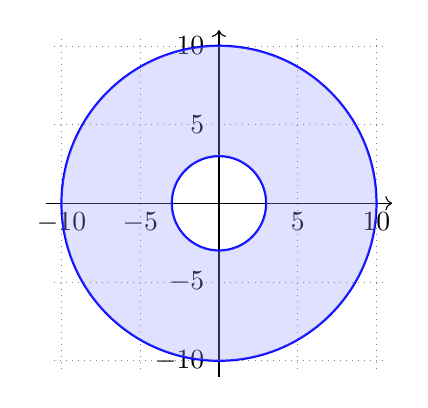
\begin{tikzpicture}[scale=.2]
	\draw[step=5cm, gray, very thin, dotted] (-10.5,-10.5) grid (10.5,10.5);
	\foreach \x/\xtext in {-10,-5,5,10}
		\draw (\x,-1pt) -- (\x, 1pt) node[anchor=north] {$\xtext$};
	\foreach \y/\ytext in {-10,-5,5,10}
		\draw (-1pt, \y) -- (1pt, \y) node[anchor=east, left=2pt] {$\ytext$};
	\draw[->] (-11,0) -- (11,0);
	\draw[->] (0,-11) -- (0,11);
	\draw[thick, blue] (0,0) circle [radius=3];
	\draw[thick, blue] (0,0) circle [radius=10];
	\fill[blue!40, opacity=.3, even odd rule] (0,0) circle [radius=3] (0,0) circle [radius=10];
\end{tikzpicture}
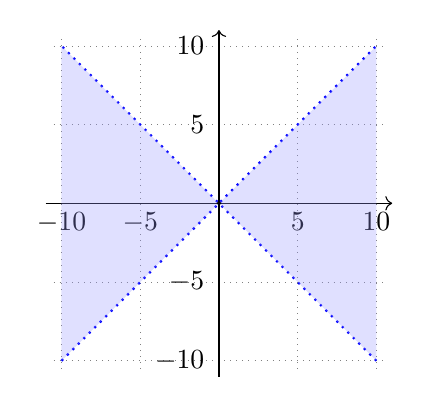
\begin{tikzpicture}[scale=.2]
	\draw[step=5cm, gray, very thin, dotted] (-10.5,-10.5) grid (10.5,10.5);
	\foreach \x/\xtext in {-10,-5,5,10}
		\draw (\x,-1pt) -- (\x, 1pt) node[anchor=north] {$\xtext$};
	\foreach \y/\ytext in {-10,-5,5,10}
		\draw (-1pt, \y) -- (1pt, \y) node[anchor=east, left=2pt] {$\ytext$};
	\draw[->] (-11,0) -- (11,0);
	\draw[->] (0,-11) -- (0,11);
	\draw[thick, blue, dotted] (-10,-10) -- (10,10);
	\draw[thick, blue, dotted] (10,-10) -- (-10,10);
	\fill[blue!40, opacity=.3] (0,0) -- (10,-10) -- (10,10) -- cycle;
	\fill[blue!40, opacity=.3] (0,0) -- (-10,-10) -- (-10,10) -- cycle;
	\filldraw[black] (0,0) circle (.1);
\end{tikzpicture}
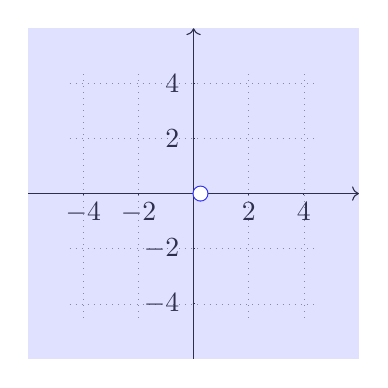
\begin{tikzpicture}[scale=.35]
	\draw[step=2cm, gray, very thin, dotted] (-4.5,-4.5) grid (4.5,4.5);
	\foreach \x/\xtext in {-4,-2,2,4}
		\draw (\x,-1pt) -- (\x, 1pt) node[anchor=north] {$\xtext$};
	\foreach \y/\ytext in {-4,-2,2,4}
		\draw (-1pt, \y) -- (1pt, \y) node[anchor=east, left=2pt] {$\ytext$};
	\draw[->] (-6,0) -- (6,0);
	\draw[->] (0,-6) -- (0,6);
	\draw[thick, blue] (0.25,0) circle [radius=0.25];
	\fill[blue!40, opacity=.3] (-6,-6) rectangle (6,6);
	\fill[white] (.25,0) circle (.25);
\end{tikzpicture}
\end{figure}
\end{lösung}
Eine weitere sehr wichtige Ungleichung wollen wir zur Übung beweisen:
\begin{satz}{Cauchy-Schwarz-Ungleichung}{cauchyschwarz}
Seien $x_1, \dots, x_n, y_1, \dots, y_n \in \C$ endlich viele komplexe Zahlen. Dann gilt die \textbf{Cauchy-Schwarz-Ungleichung}
\begin{equation}
\left| \sum_{i=1}^n x_i \overline{y}_i\right|^2 \leq \sum_{i=1}^n |x_i|^2 \sum_{i=1}^n |y_i|^2.
\end{equation}
\end{satz}
\begin{beweis}
Für den Beweis brauchen wir zwei Vorüberlegungen. Erst einmal bemerken wir, dass die Gleichung immer gilt, wenn $\sum_i |x_i|^2 \sum_i|y_i|^2 = 0$, da dann alle $x_i$ oder alle $y_i$ verschwinden müssen. Wir müssen den Beweis also nur noch für $\sum_i |x_i|^2 \sum_i|y_i|^2 > 0$ führen. Die andere Vorüberlegung ist etwas technisch\footnote{Wer denkt, die folgenden Umformungen fielen vom Himmel, kann versuchen, es von vorn nach hinten anzugehen. Dann ist es viel offensichtlicher.} Seien $\alpha, \beta, \gamma, \delta \in \R$. Da Quadrate reeller Zahlen immer positiv sind, stellen wir fest:
\begin{align*}
0 \leq (\alpha \delta- \beta \gamma)^2 &= \alpha^2\delta^2 + \beta^2 \gamma^2 -2\alpha \beta \gamma \delta\\
&= \blue{\alpha^2 \beta^2 - \alpha^2 \beta^2 + \gamma^2 \delta^2 - \gamma^2 \delta^2} +\alpha^2\delta^2 + \beta^2 \gamma^2 -2\alpha \beta \gamma \delta\\
&= (\alpha^2 + \gamma^2)(\beta^2+\delta^2) - (\alpha^2 \beta^2 + \gamma^2 \delta^2 + 2 \alpha \beta \gamma \delta)\\
&= (\alpha^2 + \gamma^2)(\beta^2+\delta^2) - (\alpha \beta + \gamma \delta)^2.
\end{align*}
Umstellen liefert nun eine Ungleichung, derer wir uns später bedienen:
\begin{equation}
(\ast)\, (\alpha \beta + \gamma \delta)^2 \leq (\alpha^2 + \gamma^2)(\beta^2+\delta^2).
\end{equation}
Nun beweisen wir endlich die Ungleichung mit vollständiger Induktion:\\
Für den Induktionsanfang brauchen wir nur (M2):
\begin{equation}
|x\overline{y}|^2 = (|x||\overline{y}|)^2 = |x|^2|y|^2.
\end{equation}
Hier gilt sogar Gleichheit. Die Induktionsvoraussetzung (IV) ist, dass die Aussage für $n-1$ gezeigt ist. Da beide Seiten positiv sind, können wir in der IV die Wurzel ziehen:
\begin{equation}
\left| \sum_{i=1}^{n-1} x_i \overline{y}_i\right| \leq \sqrt{\sum_{i=1}^{n-1} |x_i|^2} \sqrt{\sum_{i=1}^{n-1} |y_i|^2}.
\end{equation}
Für den Induktionsschritt müssen wir die Aussage für $n$ beweisen. Das geht nun relativ schnell:
\begin{align*}
\left| \sum_{i=1}^n x_i \overline{y}_i\right| &= \left| x_n \overline{y}_n + \sum_{i=1}^{n-1} x_i \overline{y}_i\right|\leq |x_n \overline{y}_n| + \left| \sum_{i=1}^{n-1} x_i \overline{y}_i\right|\\
&\leq^\text{\red{IV}} |x_n| |y_n| + \sqrt{\sum_{i=1}^{n-1} |x_i|^2} \sqrt{\sum_{i=1}^{n-1} |y_i|^2} \leq^{\red{(\ast)}} \sqrt{\sum_{i=1}^{n} |x_i|^2} \sqrt{\sum_{i=1}^{n} |y_i|^2}
\end{align*}
Im ersten Schritt haben wir die Dreiecksungleichung ausgenutzt, gefolgt von der Induktionsvoraussetzung. Den letzten Schritt können wir mit unserer Ungleichung $(\ast)$ direkt folgern, indem wir $\alpha:=|x_n|$, $\beta:= |y_n|$, $\gamma:= \sqrt{\sum_{i=1}^{n-1} |x_i|^2}$ und $\delta :=\sqrt{\sum_{i=1}^{n-1} |y_i|^2}$ setzen.
\end{beweis}
\printindex
\end{document}
